\newpage
\phantomsection
{\bfseries IRSTI 20.15.05}
\hfill {\bfseries \href{https://doi.org/10.58805/kazutb.v.2.23-483}{https://doi.org/10.58805/kazutb.v.2.23-483}}

\sectionwithauthors{N.K.Yurkov}{METHODOLOGY FOR IMPROVING THE CYBER THREAT PROTECTION SYSTEM}

\begin{center}
{\bfseries N.K.Yurkov}

Penza State University, Penza, Russia,

e-mail: Yurkov\_nk@mail.ru
\end{center}

The article presents the results of a study of the enterprise
information security system and the development of proposals for its
implementation. The article considers security as a system that includes
tools and processes used by organizations to protect information. This
includes policy settings that prevent unauthorized persons from
accessing business or personal information. Information security is
positioned as a growing and developing industry, covering a wide range
from network and infrastructure protection to testing and auditing.

The article analyzed IT products designed to ensure information security
that are used in small and medium-sized businesses, explored problem
areas and current applications that entrepreneurs use.

One of the most pressing problems in the IT industry today, in the era
of big data, is the rapid growth of the volume of unstructured content.
Virtually every corporate data center (Docs) has file servers, corporate
portals, Microsoft Exchange folders, network and cloud storage locations
that contain many documents, including the content of important
information. In addition, the repeated increase in volume and the
growing variety of information stored and processed significantly
complicates the task of managing this data.

{\bfseries Keywords:} information security, tools, processes, systems and
networks, cyber attacks, phishing, artificial intelligence, machine
learning.

\begin{center}
{\large\bfseries МЕТОДОЛОГИЯ ПОВЫШЕНИЯ СИСТЕМЫ ЗАЩИТЫ ОТ КИБЕРУГРОЗ}

{\bfseries Н.К.Юрков}

Пензенский государственный университет, Пенза, Россия,

e-mail: Yurkov\_nk@mail.ru
\end{center}

В статье представлены результаты исследования системы информационной
безопасности предприятия и разработаны предложения по ее внедрению. В
статье безопасность рассматривается как система, включающая инструменты
и процессы, используемые организациями для защиты информации. Сюда
входят настройка политики предотвращения доступа посторонних лиц к
деловой или личной информации. Информационная безопасность
позиционируется как растущая и развивающаяся отрасль, охватывающая
широкий спектр от защиты сетей и инфраструктуры до тестирования и
аудита.

В статье проанализированы ИТ-продукты, предназначенные для обеспечения
информационной безопасности, которые используются в малом и среднем
бизнесе, рассмотрены проблемные области и актуальные приложения,
которыми пользуются предприниматели.

Одной из самых актуальных проблем IT-индустрии сегодня, в эпоху больших
данных, является стремительный рост объема неструктурированного
контента. Практически в каждом корпоративном центре обработки данных
(Docs) есть файловые серверы, корпоративные порталы, папки Microsoft
Exchange, сетевые и облачные хранилища, содержащие множество документов,
в том числе важную информацию. Кроме того, многократное увеличение
объема и растущее разнообразие хранимой и обрабатываемой информации
значительно усложняет задачу управления этими данными.

{\bfseries Ключевые слова:} информационная безопасность, инструменты,
процессы, системы и сети, кибератаки, фишинг, искусственный интеллект,
машинное обучение.
\newpage
\begin{center}
{\large\bfseries КИБЕРҚАУІПТЕРДЕН ҚОРҒАУ ЖҮЙЕСІН ЖАҚСАРТУ ӘДІСТЕМЕСІ}

{\bfseries Н.К. Юрков}

Пенза Мемлекеттік Университеті, Пенза, Ресей

e-mail: Yurkov\_nk@mail.ru
\end{center}

Мақалада кәсіпорынның ақпараттық қауіпсіздік жүйесін зерттеу нәтижелері
және оны жүзеге асыру бойынша ұсыныстар әзірлеу ұсынылған. Мақалада
қауіпсіздік ақпаратты қорғау үшін ұйымдар пайдаланатын құралдар мен
процестерді қамтитын жүйе ретінде қарастырылады. Бұған бөгде адамдардың
іскерлік немесе жеке ақпаратқа қол жеткізуіне жол бермейтін саясат
параметрлері кіреді. Ақпараттық қауіпсіздік желіні және инфрақұрылымды
қорғаудан бастап тестілеу мен аудитке дейінгі кең ауқымды қамтитын өсіп
келе жатқан және дамып келе жатқан сала ретінде орналасқан.

Мақалада шағын және орта бизнесте қолданылатын ақпараттық қауіпсіздікті
қамтамасыз етуге арналған АТ өнімдеріне талдау жасалды, проблемалық
аймақтар мен кәсіпкерлер қолданатын ағымдағы қосымшалар зерттелді.

Бүгінгі таңда IT индустриясындағы ең өзекті мәселелердің бірі, үлкен
деректер дәуірінде құрылымданбаған мазмұн көлемінің қарқынды өсуі болып
табылады. Іс жүзінде әрбір корпоративтік деректер орталығында (Docs)
көптеген құжаттарды, соның ішінде маңызды ақпараттың мазмұнын қамтитын
файлдық серверлер, корпоративтік порталдар, Microsoft Exchange
қалталары, желілік және бұлттық сақтау орындары бар. Сонымен қатар,
көлемнің бірнеше рет ұлғаюы және сақталатын және өңделетін ақпараттың
өсіп келе жатқан әртүрлілігі бұл деректерді басқару міндетін едәуір
қиындатады.

{\bfseries Түйін сөздер:} ақпараттық қауіпсіздік, құралдар, процестер,
жүйелер мен желілер, кибершабуылдар, фишинг, жасанды интеллект,
машиналық оқыту.

\begin{multicols}{2}
{\bfseries Introduction.} For the development of the concept of ensuring
information security (IC), Information is understood as data that is
available for collection, storage, processing (editing, converting), use
and transmission in various ways, including in computer networks and
other information systems. Such information has a high value and can
become the object of encroachment by third parties.the desire to protect
information from threats is the basis for the creation of information
security systems.

Information Security differs from cybersecurity in its scope and
purpose. The two terms are often used interchangeably, although it can
be said more precisely that cybersecurity is a subcategory of
Information Security. Information security is a broad field that covers
many areas, such as physical security, endpoint security, data
encryption, and network security. It is also closely related to
Information Security, which protects information from threats such as
natural disasters and server failures.

Cybersecurity is primarily focused on combating threats related to
technology, as well as methods and tools that allow you to avoid or
minimize their consequences. Another adjacent category is data security,
which aims to protect the organization\textquotesingle s information
from accidentally or in a harmful way falling into the hands of
unauthorized persons.

Creating an effective security policy and taking measures to implement
it is an important step towards preventing and reducing security
threats. For a policy to be truly effective, it needs to be updated
frequently, taking into account changes in the company, new threats,
conclusions made on the basis of previous violations, as well as changes
in systems and protective equipment. Information security doctrines.

It is also closely related to Information Security, which protects
information from threats such as natural disasters and server failures.

Cybersecurity is primarily focused on combating threats related to
technology, as well as methods and tools that allow you to avoid or
minimize their consequences. Another adjacent category is data security,
which aims to protect the organization\textquotesingle s information
from accidentally or in a harmful way falling into the hands of
unauthorized persons.

Make your information security strategy practical and reasonable. To
meet the needs and urgency of the various units of the organization, it
is necessary to introduce an exclusion system with an approval process
that allows units or individuals to retreat from the rules in specific
situations. There are hundreds of categories of information security
threats and millions of known threat vectors. Below we will consider
some of the main threats that are a priority for the security groups of
modern enterprises.

{\bfseries Methods and materials.} Before developing an information
security strategy, it is necessary to adopt the basic definition of the
concept, which allows you to apply certain methods and methods of
protection. Industry practitioners propose to understand as information
security the stable state of protection of Information, its carriers and
infrastructure, ensuring the integrity and stability of
information-related processes to the intentional or unintentional impact
of a natural and artificial nature. Effects are classified as white
threats that can harm subjects of information relations.

The basic principles of information security are confidentiality,
integrity and accessibility. Each element of the information security
program should be designed to implement one or more of these principles.
Together they are called Triads. Privacy measures are designed to
prevent unauthorized disclosure of information. The purpose of the
principle of confidentiality is to keep personal information
confidential and ensure that it is visible and accessible only to those
who own or need it to perform their organizational functions {[}1{]}.

In the theory of information security, the subjects of information are
understood as owners and users of information, and users are not only on
an ongoing basis (employees), but also users who apply to databases in
individual cases, for example, government agencies requesting
information. In some cases, for example, in the standards of Bank JSC,
shareholders -- legal entities that own certain data belong to the
owners of information.

From the point of view of the basics of JSC, the support infrastructure
includes computers, networks, telecommunications equipment, premises,
life support systems, personnel. When analyzing security, it is
necessary to study all elements of systems, paying special attention to
personnel as carriers of most internal threats (fig.1).
\end{multicols}

\begin{figure}[H]
	\centering
	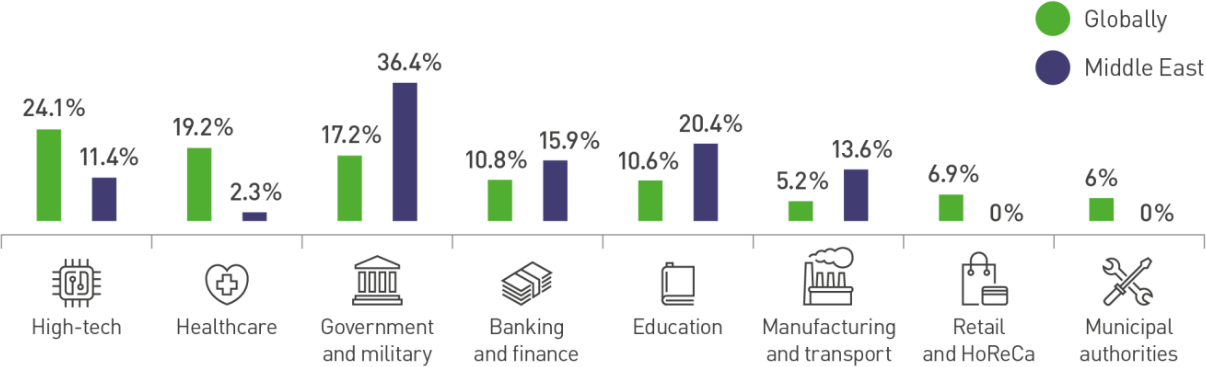
\includegraphics[width=0.8\textwidth]{assets/63}
	\caption*{Figure 1 -- Statistics of incidents related to Information Security}
\end{figure}

\begin{multicols}{2}
For information security management and damage assessment, a suitability
characteristic is used, so that damage is defined as acceptable or
unacceptable. It is useful for each company to establish its own
criteria for the admissibility of damage in monetary terms or, for
example, in the form of reputational damage. Government agencies may
adopt other characteristics, such as influencing the management process
or indicating the degree of harm to the life and health of citizens. The
criteria for the importance, significance and value of information may
change during the life cycle of the information array, so they must be
revised in a timely manne {[}2{]}.

An information threat in a narrow sense is recognized as an objective
opportunity to influence an object of protection, which can lead to
leakage, theft, disclosure or dissemination of information. In a broad
sense, AK -- threats include directed effects of an informational
nature, the purpose of which is to harm the state, organization,
individual. Such threats include, for example, slander, deliberate
misleading, incorrect advertising.

Today, one of the biggest threats to business is the leakage of
confidential information. As a rule, the source of such threats is
unscrupulous employees of insider companies {[}3{]}. Uncontrolled use of
the internet (social networks, instant messengers, personal mail) can
lead to leakage of confidential information, which, in turn, causes
significant damage to business. In addition, the headache of any leader
is employee fraud. Various rollbacks and gray schemes not only cause
one-time economic damage, but also have a serious impact on the
reputation of the organization for a long time, which leads to even more
financial losses (fig.2).
\end{multicols}

\begin{figure}[H]
	\centering
	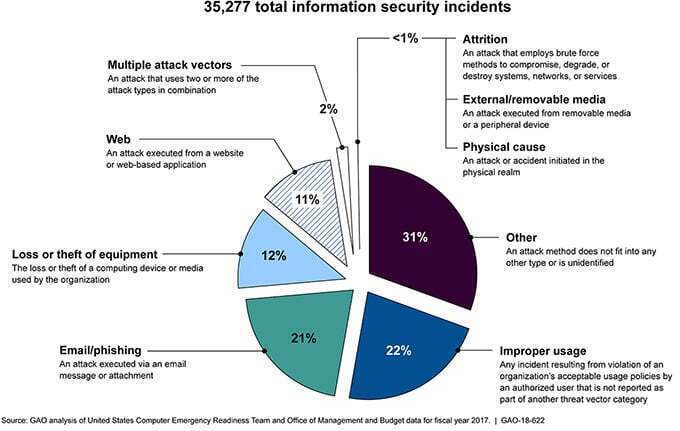
\includegraphics[width=0.6\textwidth]{assets/64}
	\caption*{Figure 2 - Jackson Diagram}
\end{figure}

\begin{multicols}{2}
If a manager does not know how his employees work, then his business
cannot be profitable, productive and protected. In such a situation,
accounting for working hours and control over employees is not just a
necessary, but a vital measure. Many employers are interested in
monitoring the behavior of the employee in the workplace. Therefore,
today more and more companies are paying attention to employee
efficiency monitoring systems that help solve complex problems in
preventing information leaks, investigating incidents, as well as
monitoring business processes and how employees use their working time
{[}4{]}.

The typical architecture of such systems assumes the presence of a
server, database, agent and administrator console. At the same time, the
following can be distinguished: systems in a bold client, the server and
agents must necessarily be in the local network, solutions that allow
you to work with agents in other networks, a cloud --- based
solution-the database is in the vendor, and agents are not connected to
the local network, management and viewing is carried out through the web
console. Data breach (fig.3).
\end{multicols}

\begin{figure}[H]
	\centering
	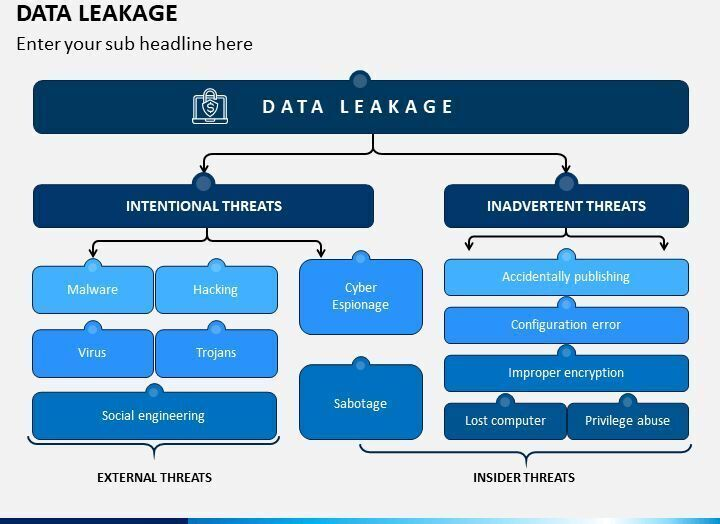
\includegraphics[width=0.7\textwidth]{assets/65}
	\caption*{Figure 3 - Data breach}
\end{figure}

\begin{multicols}{2}
In addition to tasks related to monitoring user efficiency, monitoring
systems solve a number of problems related to monitoring data channels
and preventing leaks of confidential information - systems can
successfully perform the main, most demanded part of DLP functions and
monitor leaks of confidential information related to monitoring all data
channels and working with external devices {[}5{]}. In the system Event
Tracking part, you can monitor the use of the software registry,
hardware, ports, programs and websites (fig.4).
\end{multicols}

\begin{figure}[H]
	\centering
	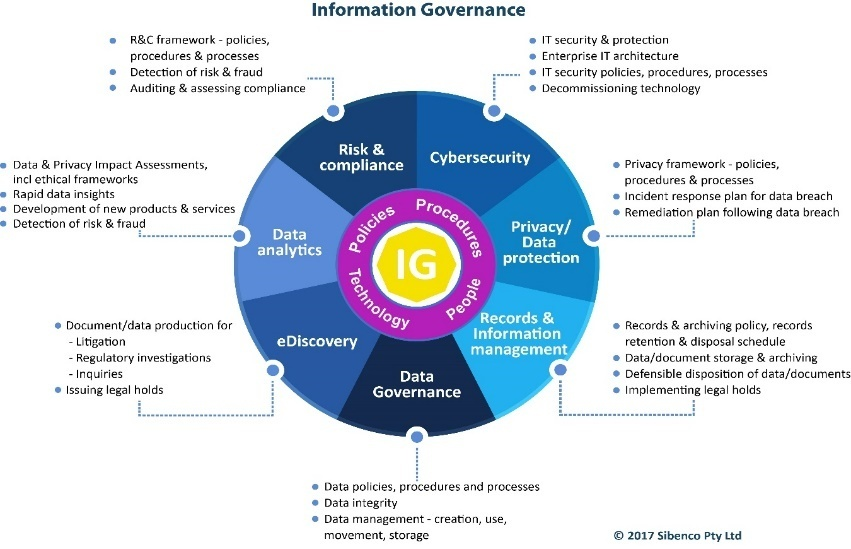
\includegraphics[width=0.9\textwidth]{assets/66}
	\caption*{Figure 4 - Information management pie chart}
\end{figure}

\begin{multicols}{2}
Often, business owners, department heads and it and IT specialists find
it difficult to answer questions: what information is stored on which
servers, who is the owner of this data, who uses them and how.
Inefficient information management leads to an increase in risks for
business: the storage of personal data and other confidential
information on publicly available information resources, the appearance
of suspicious encrypted user archives, violation of the policy of
accessing important information, etc.

{\bfseries Results and Discussion.} In the data-Centric Audit and
Protection 2021 Market Guide report, the research company Gartner
analyzed the global data-centric Audit and Protection market and listed
its representatives by dividing them into several segments: Database

Management Solutions (DataBase), file Storage solutions (File Storage),
solutions for working with Big Data, Control solutions for SaaS and IaaS
(fig.5).

According to the Data Management Market Global Forecast Report for 2021
by Components (solutions and services), applications (event Regulation
Management, Risk Management, Sales and marketing optimization),
deployment, vertical, business functions and regions published by
Marketsandmarkets, the data management market is projected to grow at
доллардан 863.2 million (2016).) up to 2234.7 million dollars for 2021.
At the same time, the average annual growth rate (CARG) for the forecast
period is 21\%. The report noted that the main factors driving the data
management market are the need for regulators to comply with security
requirements, as well as improving and maintaining strategic risk
management. According to the forecast for 2016-2020, the main share of
the data management market is expected to belong to North American
countries.
\end{multicols}

\begin{figure}[H]
	\centering
	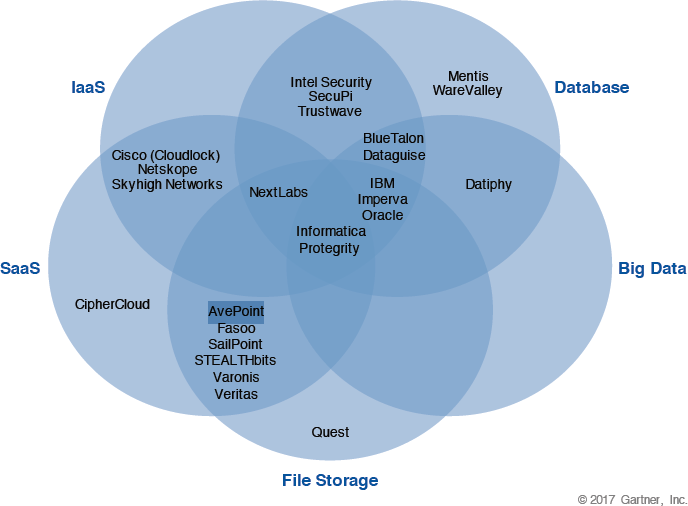
\includegraphics[width=0.6\textwidth]{assets/67}
	\caption*{Figure 5 - Gartner dcap market vendor allocation chart}
\end{figure}

\begin{multicols}{2}
The Russian data Access Governance market is still in the development
stage. It is mainly represented by solutions from Western sellers.
Russian solutions can only include the Nautilus product from cross
Technologies, which is an OEM solution for the datadvantage module
manufactured by Varonis Systems with a completely Russian-language
interface. At the moment, an application is being considered for the
inclusion of this solution in the Russian software registry. It is also
worth noting that some solutions of the IDM class have the functionality
of dag solutions, in part, in the part of managing access to data stored
in Microsoft SharePoint shared folders and portals{[}6{]}. These are
systems such as 1idm (more details with the product can be found here)
and cube (more details with the product can be found here)

Before talking about the market for DLP systems, you need to decide what
it means when it comes to such solutions. DLP systems are usually
understood as software products that protect organizations from leaks of
confidential information. The abbreviation DLP itself stands for data
Leak Prevention, that is, it prevents data leakage (fig.6).
\end{multicols}

\begin{figure}[H]
	\centering
	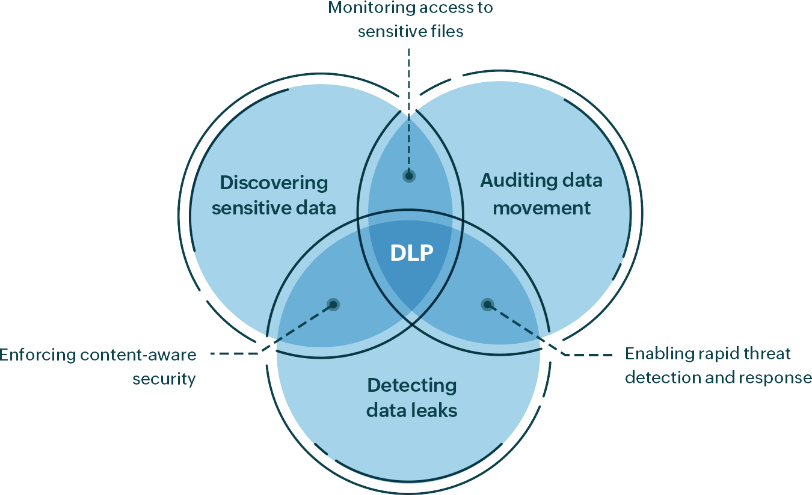
\includegraphics[width=0.6\textwidth]{assets/68}
	\caption*{Figure 6 - DLP system}
\end{figure}

\begin{multicols}{2}
Regularly scan the organization\textquotesingle s IP addresses from the
internet to make sure that the servers and services that should be
available to the global network only on the company\textquotesingle s
local network are not "visible". If an unnecessary service unexpectedly
"shines" on the Internet, act quickly to block access to it from the
outside. If the service is really available from the internet, regularly
apply security updates to it and protect it with MFA {[}7{]}. These
measures are especially important for hackers \textquotesingle{}
favorite objects such as web management console, RDP, Telnet/SSH, SMB,
SNMP, FTP. Assume that any service visible from the internet scans every
day for vulnerabilities, simple passwords and other problems (fig.7).
\end{multicols}

\begin{figure}[H]
	\centering
	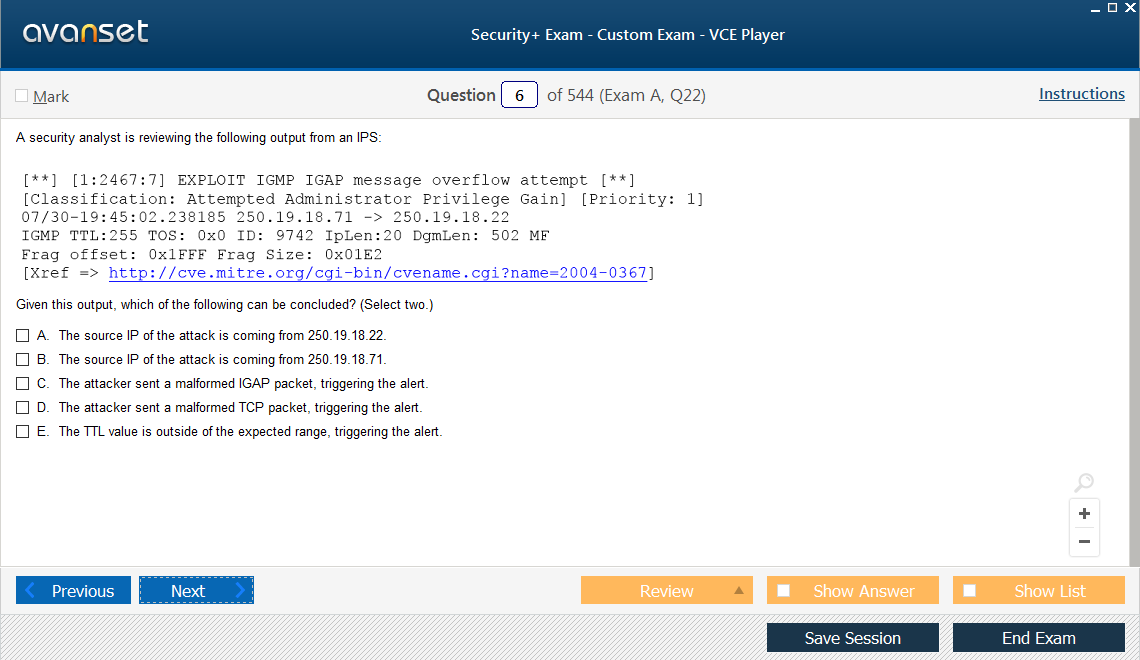
\includegraphics[width=0.8\textwidth]{assets/69}
	\caption*{Figure 7 - Analytics}
\end{figure}

\begin{multicols}{2}
Double-check all the information that" technical support"," security
service " and other departments of banks, official authorities or
representatives of your work have notified you by phone. Read the app
reviews before downloading them. Check out our posts on the five signs
of online fraud and tips on how to recognize it. Install a reliable
protection solution.

{\bfseries Conclusion.} In the process of writing the article, the tasks of
analyzing the effectiveness of the enterprise security system and
increasing it were solved. The essence of international security and
socio-political phenomena such as "cyberterrorism" and "cybersecurity"
were considered. The tasks of cyberterrorism in the modern period were
studied. The most important areas of cybersecurity policy have been
resolved. An overview of the state of the artificial intelligence
segment in Information Security allows us to draw the following
conclusions: artificial intelligence makes a significant contribution to
the fight against modern information threats. In particular, in most
cases, the introduction of artificial intelligence technologies into the
organization\textquotesingle s Information Security reduces the time for
identifying problems and responding to events, as well as personnel
management costs. Users note an increase in the efficiency of detecting
unknown threats, as well as the speed of analyzing and detecting
malicious activity in endpoints and applications. Cumulative investments
in companies that develop information security products using artificial
intelligence technologies will amount to долларды 3,749 million at the
end of 2022. At the same time, the global market for information
security products using AI technologies will reach 3 30 billion in 2025
with an annual growth of 23\%.
\end{multicols}

\begin{center}
{\bfseries References}
\end{center}

\begin{noparindent}
1. A. Yu. Puchkov, A.M. Sokolov, S. S. Shirokov, N. N. Prokimnov
Algorithm for identifying threats to information security in distributed
multiservice networks of government bodies// Applied Informatics,
2023.-Vol.18(2)- P.85-102. DOI 10.37791/2687-0649-2023-18-2-85-102

2. Belov A. S. Modernizacija sistemy informacionnoj bezopasnosti =
Modernization of the Information Security System: The Approach to
Determining the Frequency: podhod k opredeleniju periodichnosti / A. S.
Belov, M. M. Dobryshin, D. E. Shugurov // Zashhita informacii. Insajd. -
2022. - № 4. - S. 76-80

3.Vasil\textquotesingle ev V.I., Vul\textquotesingle fin A.M.,
Kuchkarova N.V. Ocenka sovremennyh ugroz informacionnoj

bezopasnosti s ispol\textquotesingle zovaniem transformatornyh
tehnologij/ Voprosy kiberbezopasnos-

ti, 2022.- № 2.- P.27-38. DOI 10.21681/2311-3456-2022-2-27-38

4. Gladkih A. V. Metody zashhity ot DDoS --atak v
intellektual\textquotesingle nyh setjah // Cifrovaja transformacija
obshhestva i informacionnaja bezopasnost\textquotesingle: materialy
Vseross. nauch.-prakt. konf. (Ekaterinburg, 18 maja 2022 g.) -
Ekaterinburg, 2022. - S. 3-5.

5. Gladkov A. N.,Gorjachev S.N., Kobjakov N.S. Vizualizacija kiberugroz
kak aspekt formirova-

nija kompetencij v oblasti informacionnoj bezopasnosti= Visualization of
Cyber Threats as an Aspect of the Formation of Competencies in the field
of Information Security // Zashhita informacii. Insajd. - 2023. - № 1. -
S. 32-37.

6. Golubev G.D. Obzor bezopasnosti malomoshhnyh
global\textquotesingle nyh setej: ugrozy, problemy i
potencial\textquotesingle nye reshenija // Cifrovaja transformacija
obshhestva i informacionnaja bezopasnost\textquotesingle: materialy
Vseross. nauch.-prakt. konf. (Ekaterinburg, 18 maja 2022 g.) -
Ekaterinburg, 2022.- S.5-10

7. Doguchaeva S.M. Analiz sovremennyh problem informacionnoj
bezopasnosti v rossijskih kompanijah / S. M. Doguchaeva // Risk:
resursy, informacija, snabzhenie, konkurencija.- 2022. -№ 2. -S. 65--68.
EDN JXIBRK~
\end{noparindent}

\emph{{\bfseries Author information}}

\begin{noparindent}
Yurkov N.K.- Yurkov N.K.-Doctor of Technical Sciences, Professor, Penza
State University, Penza, Russia, e-mail:Yurkov\_nk@mail.ru
\end{noparindent}

\emph{{\bfseries Сведение об авторе}}

\begin{noparindent}
Юрков Н.К.-доктор технических наук, профессор, Пензенский
государственный университет, Пенза, Россия, e-mail:Yurkov\_nk@mail.ru
\end{noparindent}
